\subsection{Positive Selection Inference}
\label{sec:selection-inference}

This section presents a proposed mechanism infer gene selection events and validation experiments to test it.

\begin{sidewaysfigure}
  \centering
  \begin{minipage}{.7\textwidth} % adjust the width as needed

    \begin{minipage}{\textwidth}
      \centering
      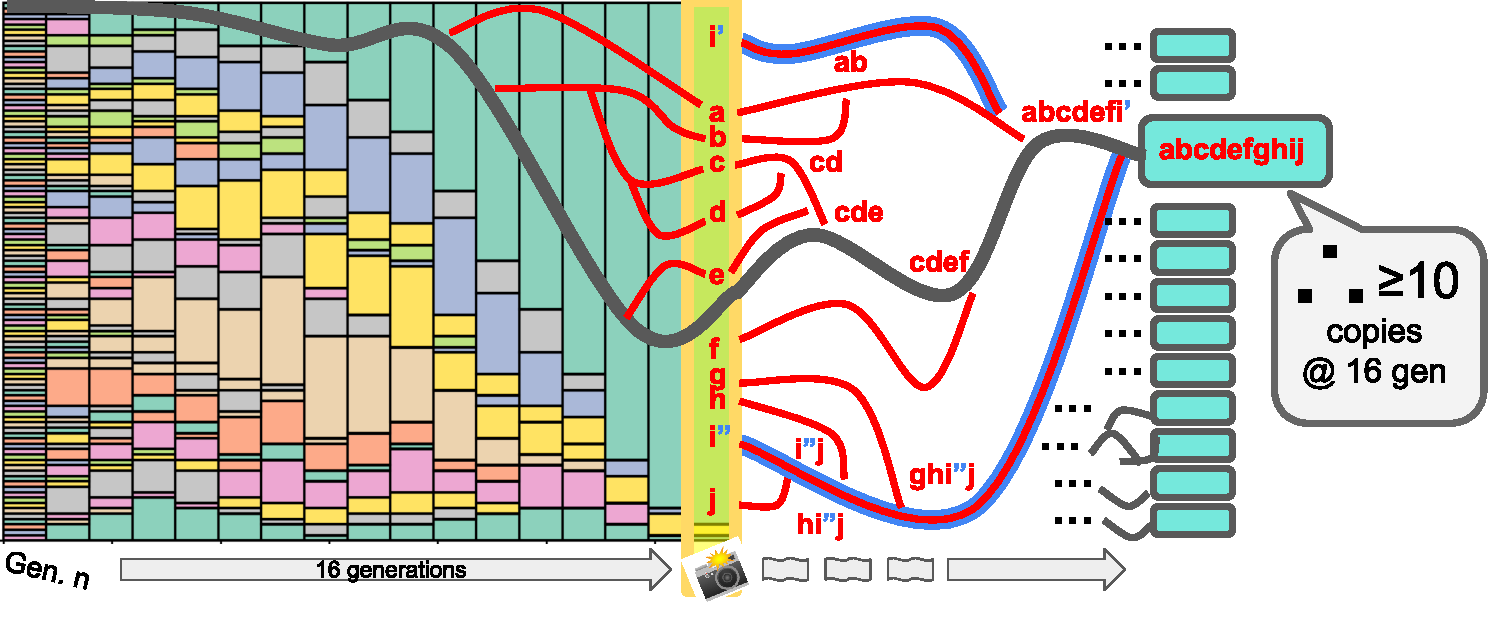
\includegraphics[height=0.30\textheight]{img/copy-count-snapshot}
      \subcaption{Cartoon depiction of delayed copy count estimation mechanism, annotated over Muller plot depicting weak selection over focal allele.
      }
      % \label{fig:ne-example-replicates:bottleneck}
    \end{minipage}%

    \vspace{1cm}

    \begin{minipage}{0.5\textwidth}
      \centering
      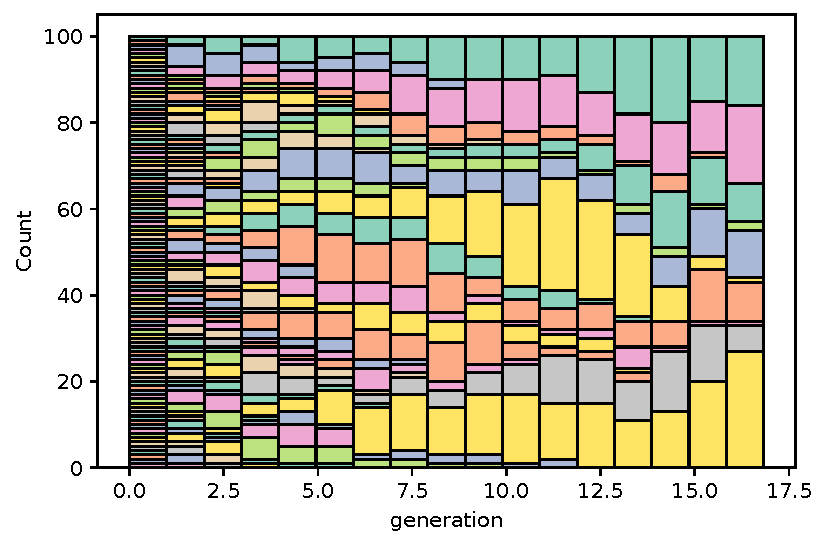
\includegraphics[height=0.2\textheight]{notebooks/notebooks/teeplots/fit=0.0+hue=clade+multiple=stack+ngen=16+npop=100+palette=set2+viz=histplot+x=generation+ext=}
      \subcaption{Muller plot depicting no selection for focal allele, ending with smaller copy count after 16 generations.}
      % \label{fig:ne-example-replicates:selection_pressure}
    \end{minipage}%
    \begin{minipage}{0.5\textwidth}
      \centering
      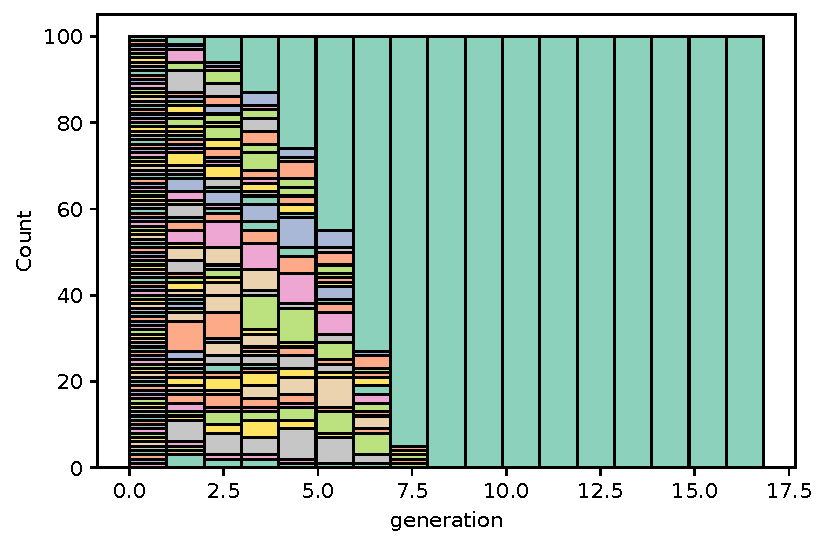
\includegraphics[height=0.2\textheight]{notebooks/notebooks/teeplots/fit=1.0+hue=clade+multiple=stack+ngen=16+npop=100+palette=set2+viz=histplot+x=generation+ext=}
      \subcaption{Muller plot depicting strong selection for focal allele, with fixation occuring before 16 generations.}
      % \label{fig:ne-example-replicates:control}
    \end{minipage}

  \end{minipage}
  \hfill % Creates horizontal space. Can also use \hspace{<len>}
  \begin{minipage}{.25\textwidth} % adjust the width as needed
    \caption{
      Proposed mechanism for detecting gene-level selection via a distributed delayed copy count estimation mechanism.
      Strata deposited at generation $n$ progress through 16 generations, with copy count of one allele growing due to selection.
      On the sixteenth generation, a ``snapshot'' is performed to set a random bit on field annotated onto each descendant differentia copy.
      In subsequent recombination events, set bits are exchanged between bit fields associated with common differentia.
      Copy count at generation $n + 16$ from can then estimated from these bit fields, with high copy count being suggestive of selection.
      Note that in this example collision between set bits $i'$ and $i"$ result in an undercount.
      This mechanism is associated with ``gene-level'' instrumentation (Figure \ref{fig:annotation-types}).
    }
    \label{fig:ne-example-replicates}
  \end{minipage}

\end{sidewaysfigure}


% notebooks/notebooks/teeplots/notebook=ne-inference+replicate=0+treatment=bottleneck+viz=plot-running-estimation+x=rank+y=population-size+ext=.pdf
%
% notebooks/notebooks/teeplots/notebook=ne-inference+replicate=0+treatment=control+viz=plot-running-estimation+x=rank+y=population-size+ext=.pdf
%
% notebooks/notebooks/teeplots/notebook=ne-inference+replicate=0+treatment=range-expansion+viz=plot-running-estimation+x=rank+y=population-size+ext=.pdf
%
% notebooks/notebooks/teeplots/notebook=ne-inference+replicate=0+treatment=selection-pressure+viz=plot-running-estimation+x=rank+y=population-size+ext=.pdf

\textbf{Inference Mechanism.}
Alleles experiencing positive selection increase in frequency.
However, allele frequency increases can also occur through drift.
The key difference between the two is the \textit{rate} of increase --- drift tends to be slower than selection, especially for large population sizes.

Selection can be differentiated from drift dynamics by capturing an estimate of copy count of each gene's descendants after a fixed number of generations $g$ elapse.
If this copy count falls in the tails of the distribution expected under a null hypothesis of pure drift dynamics, positive selection can be inferred.
Stronger positive selection will correlate with greater growth of copy count within the $g$ generation window.

The proposed mechanism uses gene-level instrumentation.
In order to record estimated copy count, each fingerprint is bundled with an additional fixed-length, zero-initialized bit field.
Each ``fingerprint'' has its own associated supplementary annotation.
The bit fields are copied verbatim to descendants along with the rest of gene annotations.

At the $g$th generation following its creation, a single bit is set at a random position of each bit field.
Recombination combines corresponding bit fields with matching fingerprints using the bitwise or operation.
In this manner, set bits propagate among the records of all gene copies that trace back to a particular founder at outset of the snapshot window.

Annotations' bit counts converge to reflect the number of gene copies present after generational delay $g$.
Figure \ref{fig:copy-count-snapshot} summarizes the overall mechaniism.
Set bits can under count of gene copies due to positional collisions between set bits or gene copy extinctions subsequent to generation $g$.
Notably, though, over count is not possible.
This conservative property ensures events would only be falsely detected due to \textit{bona fide} increases in copy count through drift, not due to instrumentation-associated error.%
\footnote{This conservative property holds under the assumption of no spurious fingerprint collision.}
Sensitivity to larger copy counts could be achieved by setting bits instead with probability $p < 1$, although this would introduce potential for instrumentation-associated copy count overestimation.

A bit field with of 8 bytes and a snapshot delay of 16 generations, by arbitrary choice, were used in experiments.
Better sensitivity to weak selection events should be achievable through longer snapshot windows and larger bit fields, but potentially at the cost of diluting signal from strong selection events.
Future work should seek a principled procedure to tailor snapshot window length and bit field widths to experimental objectives and evolution system properties.

Soft sweeps should, in principle, be detectable to some extent through this methodology, as they involve increases in copy count at faster-than-drift rates.
These are scenarios where changes in environmental conditions induce positive selection on an existing, potentially widespread allelic variant that was previously neutral \citep{hermisson2005soft}.
However, weak sweeps on very-widespread alleles that quickly reach fixation will register only a weak signal on this instrumentation because increases in copy count are spread across the large number of preexisting allele copies.
Although weak sweeps are not tested in this work, this limitation merits future consideration.

\textbf{Validation Experiment.}
A minimalistic experimental system was devised to test capability to detect detect positive selection on a novel allele.
Each individual in the population comprised a single floating-point number, representing a single focal gene.
Gene values were restricted between 0.0 and 1.0.
Fitness score was defined as the sum of the genetic value and a random number drawn from a continuous, uniform unit-valued distribution.
So, individuals' gene value corresponded directly to probabilistic fitness advantage.
For example, a value of 0.2 would give an average 20\% selective advantage.
Fitness scores for each individual were calculated once per generation and used for all tournaments.

All individuals were initialized with gene value 0.0.
At generation 50, one organism's gene value was set to either 0.0,\footnote{The smallest representable floating point value was set for fitness advantage treatment 0.0 so the introduced gene could be differentiated from the background gene.
This value was small enough as to have no meaningfully detectable effect on selection.} 0.1, or 1.0.
This operation was repeated at subsequent generations if the introduced gene value went extinct.
This procedure enabled comparison of a strong selective sweep for the gene (fitness advantage 1.0), a weaker selective sweep for the gene (fitness advantage 0.1) and a control treatment where no fitness advantage was introduced and pure drift dynamics were at play (fitness advantage 0.0).
Underlying selective sweep dynamics were measured by recording gene copy count at each generation.

Synchronous selection with tournament size 2 was performed each generation.
200 generations were simulated, with a constant population size of 400.
Crossover propagated a random parent's gene value.
No mutation was applied.
Ten independent replicates were performed of each treatment.
